71. \begin{figure}[ht!]
\center{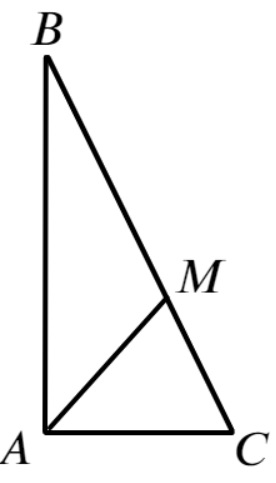
\includegraphics[scale=0.35]{g9-71.png}}
\end{figure}\\
По свойству основания биссектрисы имеем соотношение $\cfrac{AB}{AC}=\cfrac{BM}{MC}=3:1.$ Пусть $AC=x,\ AB=3x,$ тогда по теореме Пифагора $x^2+9x^2=(3+1)^2,\ x^2=\cfrac{8}{5}.$ Посчитаем площадь треугольника двумя способами: $S=\cfrac{1}{2}AD\cdot4=\cfrac{1}{2}x\cdot3x,$ откуда $4AD=3\cdot\cfrac{8}{5},\ AD=\cfrac{6}{5}.$\\
